% \chapter{Introduction}
\section{\orange{Introduction}}

In this thesis I want to investigate and discuss a certain model of cognition.
- We look at the world and learn to distinguish things. Discernment is the fundamental operator of cognition.
we create a model of the world and of ourself (res cogitans, res extensa).
- this model is like a game engine in the head, (simulation simulacrum). we have assets, etc. and using these concepts we can construct ideas, dreams, memories, reality, etc. its all made from the same stuff.






\begin{itemize}
    \item I think that we receive sensory information and compute statistical regularities over those sensory inputs. 
    \item we construct a model of internal information and of external information and separate the world from the self, with ever more fine detail. - we create a generative model (reflexive) and inference model (reasoning)
    \item we are able to extract concepts into variables (symbols) and compute using these symbols.
    \item i think that the conceptual framework has a similar architecture as any self-organizing system (holarchic)
    \item dehaene et al show some ideas of probabilistic programming etc. 
\end{itemize}



\begin{itemize}
    \item First I discuss necessary (but not sufficient) capabilities of human cognition. 
    \item Then I present a model of how to build it (PPL)
    \item And then I propose suggestions of how to improve it and build a model 
\end{itemize}


% The pervasiveness of hierarchical and self-similar structures across various domains of natural and conceptual phenomena presents a compelling landscape for interdisciplinary inquiry. From the intricate organization of biological systems to the complex architectures of cognition and cultural dynamics, this recurrent pattern suggests an underlying principle of organization that warrants a comprehensive examination. This paper delineates the parallels between these multi-scale structures, extending the discussion into the cognitive sciences, artificial intelligence, and memetics, and situating them within the meta-theoretical framework of Wilber's Integral Theory.


% Natural systems exhibit a remarkable propensity for hierarchical organization: atoms form molecules; molecules form cells; cells form tissues; tissues form organs; and organs, in turn, form organisms. This nested structure, suggestive of a fractal-like self-similarity, is not confined to physical biology but extends into the domains of language, thought, and sociocultural constructs. Herein, we explore the implications of this hierarchical paradigm as it applies to mental models, cognitive processes, and cultural transmission, drawing correlations with existing theories and literature in these fields.


% Cognitive science posits that human thought manifests in layers of increasing complexity, from fleeting thoughts to embedded ideologies. This progression echoes biological hierarchies, whereby thoughts are the elemental units, progressively organizing into complex belief systems and comprehensive worldviews. Under the lens of the Free Energy Principle, the brain's attempt to minimize surprise through a predictive hierarchical model aligns with this multilayered structure, suggesting a cognitive economy geared towards self-organization and efficiency.


% In this thesis I am researching our ability to create a representation of the world, which leads to the ability of having a representation of ourselves and gives rise to an "I". I show how the same underlying principles describe physical organisms across multiple scales and extend that to the conceptual realm.
% A few approaches are discussed and eventually a promising Bayesian approach is experimented with and analysed. 





% \info[inline]{structure to keep in mind:}
% 3 (or more, see van Gerven) Levels of Marr
% \begin{description}
%     \item[Computational] (Building a compositional hierarchical structure, FEP, LOT, Symbolic (discrete) vs Connectionist (continuous), PPL)
%     \item[Algorithmic] (Variational Inference, GFlowNets, etc.)
%     \item[Implementational] (PyTorch, GPUs, CPUs, etc.)
% \end{description}

% \begin{itemize}
%     \item Continuously asking deeper questions as we encounter them. (what is a thought, understanding, etc.)
%     \item draw out the shape of the thesis. kind of a v shape?
%     \item golden circle (why, what, how)
%     \item But \& therefore rule of matt stone and trey parker 
% \end{itemize}

% \begin{itemize}
%     \item First we present the ubiquitous principle of nested multi-scale systems.
%     \item We show them in biological systems and how a self could emerge from that. 
%     \item We show that the mind also has this structure. 
%     \item We hypothesis that imaginaria is structured in the same way. 
% \end{itemize}

\subsection{\orange{Main Contributions}}
The main contributions of this thesis are: 
\begin{itemize}
    \item I argue that the same multi-scale hierarchies that govern biological organization can be applied to the conceptual realm
    \item I develop a method of bayesian program synthesis, using GFlowNet
    \item I present the philosophical ramifications
\end{itemize}






\begin{itemize}
    \item Have a running example throughout the text.
    \item check all [sources] etc.
    \item question: should i put prompts to gpt for all capabilities in the intro? (abduction, analogies, etc.)
    \item pseudocode from other paper?
    \item number all equations?
    \item check that forward policy has $\phi$ everywehere and generative model $\theta$
    \item also check notation $\pi(s_t+1 ...)$ or $\pi(z,...)$
    \item change replay\_prob to greek letter?
    \item Check what whould be in intro vs methods. 
    \item Introduction should introduce all capabilities and also the background work. and especially tell why we introduce it.
    \item Should parameterisation section (e.g. transformer) be more detailed?
    \item LLMs should be shortened and put in back discussion (only keep relevant parts in intro)
\end{itemize}


















\subsection{\orange{Cognition}}
In the following I will introduce some necessary (but not sufficient) core concepts of human cognition and show how we can gradually build up a model that explains some of these capabilities. Then I will show how I can improve it and explain my own model FlowCoder.

\todo[inline]{poverty of the stimulus. we learn from only a few observations. }
\subsubsection{\green{World model}}

Imagine your brain as an interactive game engine. Just as a game engine generates dynamic virtual environments, complete with rules and physics that players interact with, the brain constructs a model of the real world. This model includes rules (physical laws, social norms), entities (objects, people), and interactions (how things work and relate to each other). We learn to navigate and predict our environment, constantly updating our internal model based on new experiences and information.
This analogy, introduced by Tenenbaum et al. \cite{Ullman_Spelke_Battaglia_Tenenbaum_2017, Lake_Ullman_Tenenbaum_Gershman_2017, rule_child_2020} extends beyond mere perception, encompassing imagination, dreams, and memory. Each of these cognitive functions can be seen as manifestations of the brain's ability to generate, manipulate, and explore various scenarios and possibilities within its internal model. Dreams and imaginative constructs, while seemingly detached from reality, are composed of the same 'material' as our waking perceptions – they are all products of the brain's intricate simulation capabilities. [sources]
The self, in this view, becomes both a creator and a perceiver of its subjective reality, a reality that, while grounded in the external world, is ultimately shaped by the mind's interpretative and predictive faculties.

This paradigm posits that the brain is not merely a passive recipient of sensory inputs but rather an active participant in the construction of reality. Through the lens of Bayesian inference, the brain is conceptualized as a predictive machine. It constantly generates hypotheses or predictions about the world, drawing on past experiences and current sensory data. The brain, rather than simply processing incoming sensory information, actively infers probable causal factors behind this data, effectively reverse-engineering the world. This inferential process is guided by Bayesian principles, where the brain weighs the likelihood of various hypotheses against the evidence presented by sensory inputs. The 'prediction error' – the discrepancy between these predictions and actual sensory experiences – becomes a crucial component, informing and refining the brain's model of the world. This is the premise of many Bayesian cognitive models such as the Free-Energy. Principle, (Hierarchical) Predictive Coding, Bayesian Brain Theory, and many other variants \cite{friston_free-energy_2010, friston_world_2021} [include more sources].
The concept of the 'game engine in the head' aptly encapsulates this process, suggesting that our cognitive system operates similarly to a simulation engine, continuously constructing and updating our mental representation of the world.


\todo[inline]{Talk about intuitive physics and intuitive psychology or other research of human capabilities?}

\begin{itemize}
    \item Intuitive physics etc.
\end{itemize}

\subsubsection{\green{Bayesian Model}}

The fundamental tenet of Bayesian computational cognition is that the brain interprets the world by forming probabilistic models and updates them according to Bayesian inference principles. This means the brain weighs prior beliefs (previous experiences and knowledge) and the likelihood of new sensory evidence to arrive at posterior beliefs (updated model of the world). The brain uses these posterior beliefs to make predictions about future events, thus enabling adaptive behavior.
Bayesian inference can be formalized by:
\begin{equation}\label{form:bayes}
    P(z \vert x) = \frac{P(x \vert z) \cdot P(z)}{P(x)}    
\end{equation}

Where:
% \begin{conditions*}

% \end{conditions*}
    

\begin{itemize}
    \item \( P(z \vert x) \) is the posterior probability of hypothesis or latent variable \( z \) given the observed data \( x \).
    \item \( P(x \vert z) \) is the likelihood of data \( x \) given that hypothesis \( z \) is true.
    \item \( P(z) \) is the prior probability of hypothesis \( z \).
    \item \( P(x) \) is the marginal likelihood, the probability of the data \( x \).
\end{itemize}


\subsubsection{\green{Compositionality}}
Humans possess a native capacity for meta-cognitive evaluation, instinctively gauging the reliability of their own knowledge \cite{Lake_Ullman_Tenenbaum_Gershman_2017}. Such self-assessment serves as a compass for learning, steering the acquisition of new information in a manner that refines and optimizes our cognitive architectures.
Compositionality is central to cognitive productivity and learning. It allows for the creation of infinitely varied representations from a finite set of basic elements, similar to the mind's capacity to think an endless array of thoughts or generate countless sentences. This is particularly useful in forming hierarchical structures that simplify complex relationships, thus making inductive reasoning more efficient.
In Bayesian terms, this means that the latent $z$ can be compositional and take the form of a nested hierarchical structure.


\todo[inline]{should holarchies go here?}

\subsubsection{\green{Causal Models}}
Humans are endowed with an intuitive grasp of causality, which functions as the underpinning for both predictive and counterfactual reasoning \cite{Lake_Ullman_Tenenbaum_Gershman_2017}. This enables humans to extrapolate beyond the confines of empirical data, to conjure hypothetical worlds e.g. in imagination, play, and dreaming.
A causal model typically consists of a set of variables and a set of directed edges between these variables, often represented as a Directed Acyclic Graph (DAG). The vertices in this graph denote variables, which, in this context, could be seen as cognitive states. The directed edges signify causal relationships, pointing from cause to effect.
Causal models facilitate interventions, counterfactuals, and causal inference. Intervention is the ability to model the outcome of purposeful changes, represented mathematically as "do" operations  \cite{Pearl_2018}. For example, if one were to intervene to set $X = x$, the model would enable us to compute the distribution over $Y$ post-intervention.
Counterfactual reasoning allows us to traverse back in time, in a sense, and assess alternative realities — what would have happened to $Y$ if $X$ had been different?
Pearl sees this faculty as a crucial component of human cognition \cite{Pearl_2018}.

\subsubsection{\green{Abduction}}
How do we come up with the best explanation given partial information and limited resources? This is the problem of abduction, which can be seen as a collective term to both the generation of hypotheses, in which case it is termed \textit{abduction proper}, as well as the justification of hypotheses, also termed \textit{Inference to the Best Explanation (IBE)} \cite{burks1946peirce}.
The main problem associated with abduction proper is the difficulty of assessing how one generates fitting hypotheses quickly, while ignoring all possible non-sensical hypotheses.
Inference to the Best Explanation entails: given that we already have a set of candidate hypotheses, how do we pick the best one? Furthermore, how do we define "best"? Kwisthout presents a computational model in which he characterises "best" as an explanation that maximizes both probability as well as information content while being parsimonious \cite{kwisthout2013most}.

In the Bayesian framework the marginalisation term \( P(x) \) represents the probability of the observed data, and calculating it requires integrating over all possible hypotheses. In practical terms, this means considering how each potential hypothesis might account for every piece of observed data. This is intractable. To manage this challenge, Bayesian approximation methods provide ways to approximate \( P(x) \) without needing to perform exhaustive calculations. One common approach is to use sampling methods, such as Monte Carlo methods, which estimate 
\( P(x) \) by taking random samples from the probability distributions of the hypotheses. Another approach is variational inference, which approximates the probability distributions with simpler ones that are easier to compute. [sources + for a detailed discussion see section x]. 

It is common to divide between the generative model and the recognition density.
In this Bayesian framework, the joint probability \( P(z, x) = P(x \vert z) \cdot P(z) \) is referred to as the generative model that hypothesizes how sensory data are generated by the hidden states of the world \cite{Ramstead_Kirchhoff_Friston_2020}. In other words, it specifies a joint probability distribution over sensory inputs and potential causes of those inputs. These causes can be anything from the presence of objects in the environment to more abstract concepts like social cues.
The recognition model is an approximation of the posterior \(Q(z \vert x) \approx P(z \vert x) \), the brain's inference about the state of the world given the data.
[for further discussion see ]

\subsubsection{\green{Varied Representations}}
[aristotle - it is a sign of intelligence to be able to entertain a thought without accepting it.]
Humans interpret the same data in different ways. 
Optical illusions, like the old woman/young woman or the duck/rabbit images [show link], serve as a metaphor for this phenomenon. They demonstrate how one set of data (the image) can lead to multiple interpretations. In AI, this reflects the system's capacity to process and understand information from multiple perspectives.

% \begin{itemize}
%     \item having multiple representations of the same thing. e.g. isomorphisms, Fourier/ Laplace transform
%     \item examplified by old woman/ young woman, duck/ rabbit optical iillusion
%     \item In bayesian terms it is the question of whether we infer a point estimate, e.g. maximum a posteriori (MAP) vs trying to approximate the posterior. (Show the Bayesian formula map vs post)
%     \item We can then further ask whether we have one generative model and try to optimise it or if we construct multiple world models in parallel that are constantly competing and renegotiated.
%     \item This is related to identity and essence, when are two concepts the same? when they are isomorphic?
% \end{itemize}

From a Bayesian perspective, this idea relates to the choice between seeking a singular, most probable interpretation (Maximum A Posteriori, or MAP: $\arg max P(z|x)$) and considering a range of possible interpretations (approximating the posterior distribution: $P(z|x)$). The former approach aims for a definitive answer, while the latter embraces uncertainty and variability in the data.

\subsubsection{\green{System 1 \& System 2}}
Kahneman describes two distinct systems that characterize the dual aspects of human cognition \cite{Kahneman11}:

\emph{System 1} operates automatically and quickly, with little or no effort and no sense of voluntary control. It encompasses intuitive judgments and perceptual associations — it allows for rapid, heuristic-based processing that is often subconscious.
System 1 is akin to the generative model in Bayesian inference. Just as System 1 can produce instantaneous responses and intuitions, the generative model provides immediate perceptual hypotheses and predictions that guide behavior in a fluid and dynamic manner without the need for conscious deliberation.

\emph{System 2} allocates attention to the effortful mental activities that demand it, including complex computations. It is associated with the conscious, rational mind and is deliberate, effortful, and orderly. 
The process of updating the recognition density is more reflective and can be related to the slow, controlled inference that characterizes conscious thought. Adjusting the recognition density is akin to the effortful correction or modulation of System 1's rapid predictions when errors are detected or when more complex reasoning is required.

For example, when learning to play the piano, initial efforts require conscious attention and deliberate practice to master certain phrases (System 2). Over time, as these phrases become internalized, they can be executed more automatically and intuitively (System 1). This transition illustrates how learned skills move from conscious, effortful control to intuitive, automatic execution, mirroring the interplay between the recognition density (System 2) and the generative model (System 1) in Bayesian cognition.


\subsubsection{\green{Concepts}}
Concepts, as the building blocks of thought, vary widely in their forms and representations. They range from concrete, perceivable objects such as 'a table' to abstract notions like 'love' or 'money', theoretical constructs ('the gene', 'the atom'), mathematical entities ('addition', 'multiplication'), and even non-existent entities like 'a unicorn'. This variety, as highlighted by Blouw et al. \cite{blouw2016concepts}, underscores the diverse spectrum of concepts that the human mind can conceive and manipulate.

An effective conceptual framework not only categorizes these varied forms but also explains their \emph{extension} (why a concept refers to certain things and not others) and \emph{intension} (why it describes these referents in specific ways) \cite{ball2013surfaces}. The concept space, therefore, must be understood as a multidimensional and dynamic entity, where concepts are not isolated but embedded in a rich tapestry of relationships and attributes.

Several key criteria help in mapping and understanding this concept space:

\begin{description}
    \item [Relationship Path] This refers to the connections between concepts, governed by their similarities, differences, and functional relationships. It explains how one concept is related to or can be derived from another.
    \item [Mutual Information] This criterion examines how well concepts predict each other, based on their co-occurrence and interaction in reality. It reflects the degree to which the presence or understanding of one concept informs about another.
    \item [Change Distance] This involves measuring the conceptual 'distance' or difference between two concepts. It accounts for the extent of transformation or cognitive shift required to move from one concept to another in the conceptual space.
    \item [Parameter Distance] This refers to the number of 'knobs' or minimal changes needed to transition from one concept to another. For example, determining the minimal edits or shifts needed to transform the concept of 'dog' to 'cat', or 'rock' music to 'jazz'. This concept is akin to edit distance in text or Kolmogorov complexity in information theory, offering a quantifiable measure of conceptual transformation.
\end{description}
\todo[inline]{need sources for all of these}


[kiki, bobo, other examples]
% E.g. "dog" should be closer to "canine" than to "panda".

[for further discussion see ]


\subsubsection{\green{Large Language Models}}\label{sec:llm}
\todo[inline]{This should be Concept Space not LLMs}

% show that this allows for analogical thought and reasoning
% perhaps include bit from AAPS proposal

In his recent book "What is ChatGPT doing?", Stephen Wolfram analyses the internal mechanisms of Large Language Models (LLMs) such as GPT \cite{wolfram2023chatgpt}.
LLMs are descendents of the Transformer architecture, originally introduced in 2017 by Vaswani et al. \cite{Vaswani_Shazeer_Parmar_Uszkoreit_Jones_Gomez_Kaiser_Polosukhin_2017} and are trained on massive datasets of text and code. This allows them to learn the statistical relationships between words and phrases, and to generate human-quality text, translate languages, write different kinds of creative content, and answer questions in an informative way.
Embedding is the process of converting tokens into dense vectors of numbers. These vectors represent the semantic and syntactic information about the tokens. The embedding layer is important for LLMs because it allows them to learn the relationships between tokens in a high-dimensional space.
Various levels of embeddings are encoded, which gives aggregate words, sentences, paragraphs, etc. positions in this latent space.
LLMs primarily learn and operate through next token prediction. They use statistical patterns in data to predict language use, context, and meaning, focusing on determining the next word or phrase in a sequence. This predictive training over time leads to a complex internal representation of language, enabling the model to produce responses that are grammatically correct, contextually relevant, and semantically nuanced.
Wolfram highlights that GPT doesn't have any explicit knowledge of grammar and the parse trees that govern natural language, yet they learn these nested syntax trees implicitly. 
Nonsense sentences such as Chomsky's famous example "Colorless green ideas sleep furiously" [source], or jabberwocky sentences [source], show that there is more to language than syntax. There seems to be a semantic grammar, which LLM models learn implicitly.
LLMs, through exposure to vast amounts of text containing conditional and logical structures (e.g., "if X, then Y"), develop an ability to recognize and generate logically coherent sentences. They seem to mimic forms of syllogistic reasoning, as seen in sentences like "All X are Y. This is not Y, so it's not X." (as in "All giraffes are tall. This is not tall, so it's not a giraffe."). 
It's possible that LLMs have "discovered" syllogistic logic by looking at huge amounts of text. However, when it comes to more sophisticated formal logic, they fail [source], since they learned this implicit logic by correlation and they don't "know" the actual rules of logic.
The concept space that LLMs navigate can be illustrated through analogies such as "man is to king as woman is to queen." This represents the learnt semantic space, where relationships and associations are encoded in a high-dimensional embedding space. In this space, concepts and words are positioned in such a way that their relative distances and directions encode meaningful relationships, mirroring the complexities of human language and thought.


\begin{figure}
    \centering
    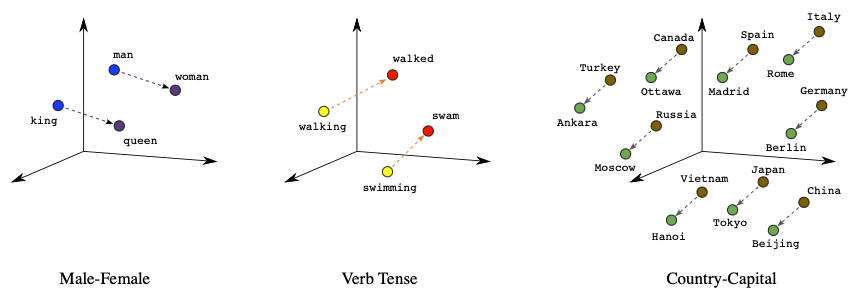
\includegraphics[width=\textwidth]{../img/embeddings_analogies.png}
    \caption{taken from google}
    \label{fig:emb_space}
\end{figure}
\todo[inline]{Explain the figure, explain vector space, dot product, etc.}




[for further discussion see ]

- holarchic direction sensory data to features, etc. 






\subsubsection{\green{Probabilistic Programming}}

Dehaene et al. posit that human cognition is uniquely characterized by its ability to form symbolic representations and recursive mental structures akin to a language of thought, enabling the creation of domain-specific conceptual systems \cite{dehaene_symbols_2022}. This cognitive ability allows for the generation of new concepts through the compositional arrangement of existing elements, a process exemplified by the derivation of geometric concepts. Cognition simplifies complex patterns into mental representations via mental compression, where the complexity of a concept is measured by the length of its mental representation as per the Minimum Description Length (MDL) principle.

Neuroscientific research indicates the presence of specialized brain circuits responsible for processing different domains of these languages of thought, with certain brain regions involved in linguistic processing and others in non-linguistic domains like mathematics and spatial reasoning [source]. The recognition of mathematical patterns is linked to the ability to detect repetition with variation, a process underpinned by specific neural areas that vary with cognitive domain.

\begin{figure}[H]
    \centering
    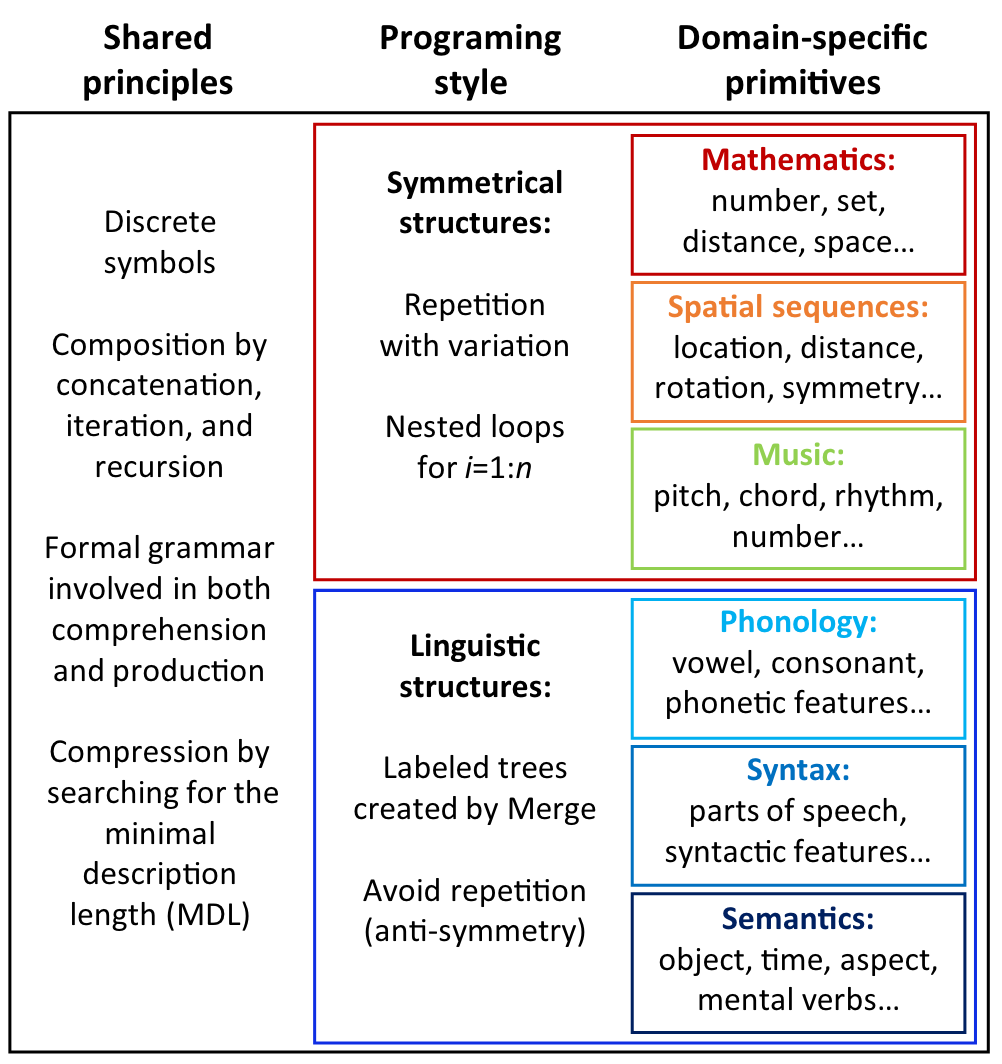
\includegraphics[width=0.7\textwidth]{../img/DSL.png}
    \caption{Image from \cite{dehaene_symbols_2022}.}
    \label{fig:DSL}
\end{figure}
\todo[inline]{Explain figure}
% Multiple mental languages, all based on symbols and recursive mental programs. Various domains of human cognition rest upon several distinct internal languages, each capable of compressing different types of inputs. Those languages share the same design principles, but differ in their primitives. Two broad styles may be distinguished: one based on the capacity to detect repetition with variation, thus appropriate for encoding symmetrical patterns and mathematical structures; and another based on asymmetrical Merge, appropriate for encoding the structures of communicative language at multiple levels. Distinct languages emerge once these general instructions are combined with domain-specific primitives.

Distinct from other primates, humans have developed the capability to use symbols in complex, rule-based systems, highlighting a unique aspect of human cognitive development. Non-human primates may associate signs with concepts; however, they do not appear to use these in the recursive, rule-based manner that humans do.

[Tenenbaum et al] posit that the brain implements mechanisms analogous to those found in probabilistic programming languages, enabling it to represent and infer the probabilistic structure of the world. Probabilistic programming provides a framework for defining complex probabilistic models and for performing inference in these models, and the hypothesis is that the brain engages in similar computational processes. [multiple sources]

Experiments show that humans do not seem to start from blank-slate but rather from rich domain knowledge [argument for primitives, more sources] \cite{lake_building_2016}. Lake et al. propose that concepts can be represented as simple stochastic programs [elaborate]. A program here can be thought of a procedure that generates more examples of the same concept. If a program would represent the concept "animal", if would generate examples such as "giraffe", "zebra", "fish", and so on. Of course, higher-level programs could produce lower-level programs, in other words, in this paradigm, the essential aspect of compositionality gives rise to a part-whole hierarchical structure, i.e. a holarchy [reference].

% The idea is that we model the world by creating programs that generate our observations \cite{rule_child_2020}.


% Roumi et al.'s experiment indeed suggest that humans may interpret and compress sequence regularities in a type of program of minimum description length (MDL) \cite{al_roumi_mental_2021}.
% Dehaene et al. further test this hypothesis and find similar results \cite{dehaene_symbols_2022}.


[the assumption we make here is that features are somehow aggregated or extracted into symbols [see \cite{garcez_neurosymbolic_2020}], primitives, along with possibly innate symbols \cite{Lake_Ullman_Tenenbaum_Gershman_2017}] 


\todo[inline]{child as a hacker}

\subsection{\red{Background}}

In the following, I will first introduce the state-of-the-art model in this regard, to present the possibilities of this framework as well as the methods used, many of which inspired my own model.

\subsubsection{\green{DreamCoder}}
One of the most successful models in this endeavor is DreamCoder - a model that synthesises programs from initial primitives and a set of tasks with the objective of learning its own domain specific language \cite{ellis_dreamcoder_2021}. The model utilises a modified version of a wake-sleep algorithm introduced by Hinton to learn a generative model and a recognition network in tandem, following the paradigm of separating the world model from the inference model \cite{hinton1995wake} [reference to earlier section, sys 1,2]. The generative model learns a probability distribution over programs while the recognition network learns to map from tasks to programs in order to perform neurally guided search over the program space. Using this recognition model, they build a parallel search algorithm which is a mixture of best-first and depth-first and enumerates programs with decreasing probabilities. See \cite{Ellis_Wong_Nye_Sable-Meyer_Cary_Morales_Hewitt_Solar-Lezama_Tenenbaum} for details.
Commonly used sub-routines, are chunked and abstracted into concepts which become more accessible. This narrows the search tree immensely and enables scalability. In sum, abstraction narrows the depth, while the recognition model narrows the breadth of the search space.

Tasks can be generative (e.g. creating an image) or conditional, (input-output relation, e.g. sorting a list).
Figure \ref{fig:conc_library}(A) shows examples of tasks across different domains. 
Figure \ref{fig:conc_library}(B) shows an example, in which the task to learn is to sort a list. On the left we see the initial primitives. The shaded region shows the learned library of concepts. On the right we see the final solution, which uses \texttt{concept15}, which itself uses previously abstracted concepts. Note the difference in the length of the program using abstracted concepts vs. only initial primitives, shown beneath.

\begin{figure*}[h]
    \centering
    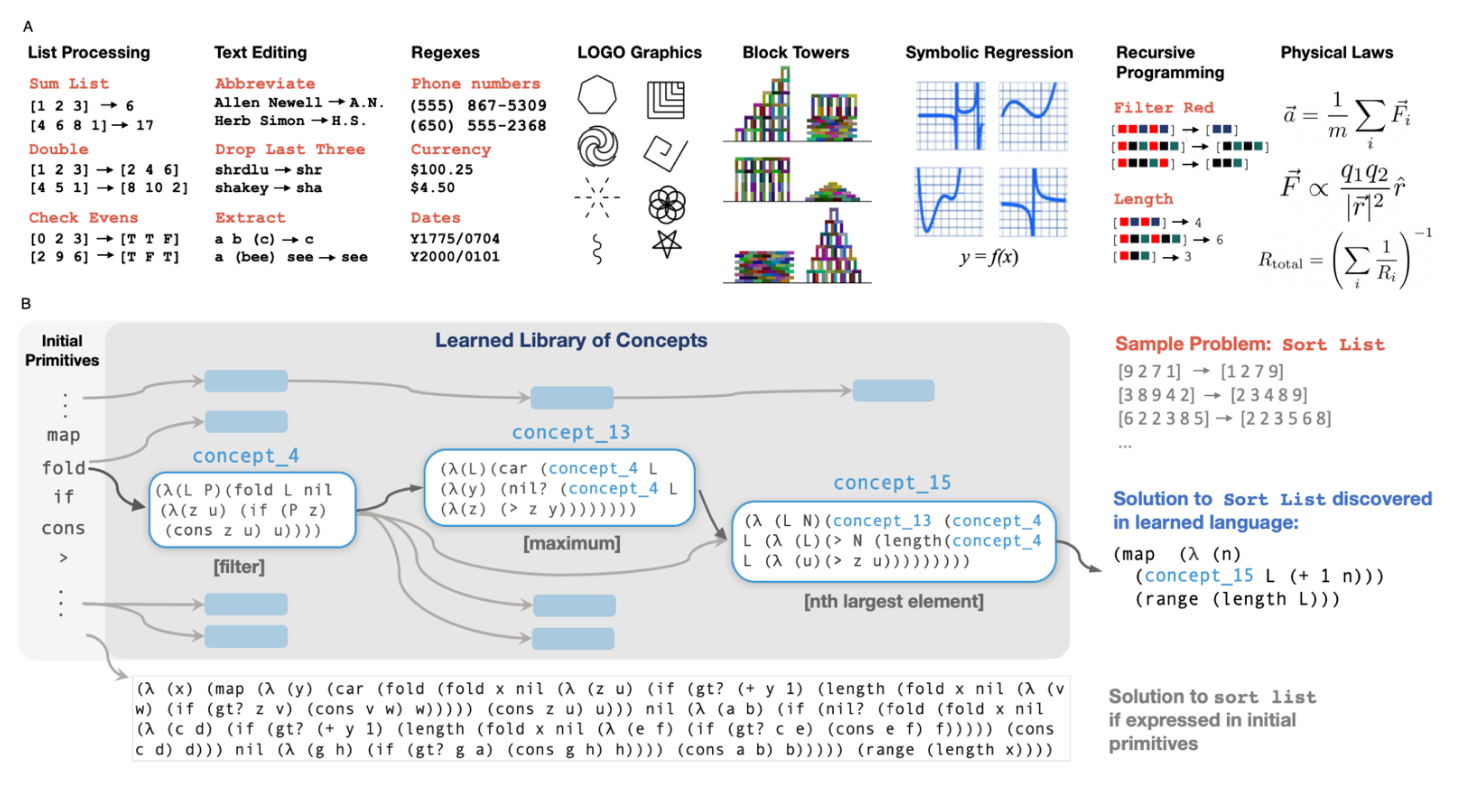
\includegraphics[width=\textwidth]{../img/conc_library.png}
    \caption{(A) 8 different domains of tasks. (B) Representation of the learned library of concepts. On the left we see the initial primitives from which the concepts in the middle region are composed. On the right we see a task as input-output relations and the found solution. On the bottom is the same solution expressed only with initial primitives. Image taken with permission from the original paper \cite{ellis_dreamcoder_2021}.}
    \label{fig:conc_library}
\end{figure*}

Formally, the overall objective of DreamCoder is to find the optimal DSL \(\mathcal{D}\), which is a set of typed \(\lambda\)-calculus expressions \todo[inline]{explain typed lambda calculus See on the representation and learning of concepts(Morales) }, along with optimal weights \( \theta \) to navigate it, such as to solve a given a set of tasks \(x \in X\).

I.e. the objective is to find the joint distribution:
\begin{equation}
    J(\mathcal{D}, \theta) = P(\mathcal{D}, \theta) \prod_{x \in X} \sum_{\rho} P(x|\rho)P(\rho|\mathcal{D},\theta) 
\end{equation}

where:
\begin{conditions*}
    P(\mathcal{D}, \theta) & Prior distribution over languages and parameters \\
    P(x|\rho) & Likelihood of task \(x \in X\) given program \(\rho\)
\end{conditions*}
\todo[inline]{whats the last term in the above formula?}
Since computing \( J(\mathcal{D}, \theta) \) entails marginalising over all programs, which is intractable, they instead marginalise over a finite beam [definition] per task \( {\mathcal{B}_x} \) which is operationalized as a lower bound on the joint density. This bound is even tighter than the ELBO [reference].
\[
    \mathcal{L}(\mathcal{D}, \theta, \{\mathcal{B}_x\}) = P(\mathcal{D}, \theta) \prod_{x \in X} \sum_{\rho \in \{\mathcal{B}_x\}} P(x|\rho)P(\rho|\mathcal{D},\theta)
\]

The model operates in three distinct phases:

\begin{description}
    \item[Wake] In the wake phase, the objective is to find the best program $\rho$ for each task $x \in X$ DreamCoder is presented with. Each task consist of one or a few ($\sim10$) examples.
    The objective is to maximize \(\mathcal{L}\) w.r.t. to the beam \(\{\mathcal{B}_x\}\)
    \item[Sleep: Abstraction] A key component of the success of DreamCoder is the refactoring of programs. In this phase, DreamCoder consolidates new abstractions from the programs it has found during the wake phase. Experiences are replayed, and commonalities between programs are found so that they can be abstracted into new concepts to use in the future. 
    In the abstraction phase \(\mathcal{L}\) w.r.t. \(\mathcal{D}\) is maximized.
    \item[Sleep: Dreaming] The objective during the dreaming phase is to train the recognition model $Q$ to perform MAP inference by both fantasies, and replays. When fantasising, programs are drawn from the learned library as a generative model. The model is then trained on the produced tasks. This ensures a large and varied data-set to learn from and encourages out-of-distribution generalisation. Replays, simply training on previously seen task-program pairs, ensures that the model improves its predictions on the actual tasks it needs to learn and doesn't forget how to solve tasks it has already solved correctly.
\end{description}

In dreaming they maximize \(\mathcal{L}\) w.r.t. \(\theta\).

\[
    \mathcal{L}_{\text{MAP}}^{\text{Replay}} = \mathbb{E}_{x\sim X} \left[ \log Q \left( \arg\max_{p \in \mathcal{B}_x} P(p|x, D, \theta)  \Big\lvert x \right) \right]
\]

\[
    \mathcal{L}_{\text{MAP}}^{\text{Fantasy}} = \mathbb{E}_{x \sim (D, \theta)} \left[ \log Q \left( \arg\max_{p} P(p|x, D, \theta) \Big\lvert x \right) \right]  
\]

\begin{description}
    \item[Parameterisation] The authors chose to optimize MAP rather than the posterior because together with their parameterisation of the recognition model, this encourages to break syntactic symmetries.

    The recognition model \(Q\) takes a task as input and outputs a 3-dimensional bigram transition matrix \(Q_{ijk}\), where \(i\) indexes possible children, \(j\) indexes possible parents and \(k\) indexes which argument of the parent is being generated. This parameterization was chosen as a balance between quality and efficiency.
    
\end{description}

% It is apparent that the abstraction phase is crucial for learning the DSL. In this project however, I want to focus on learning a good sampler. The model can subsequently always be extended to include the abstraction phase and thus expand the DSL. 



\subsubsection{\green{DeepSynth}}

In their 2021 paper, Fijalkow et al. proposed a framework called "distribution-based search", in which they investigate the difficult problem of searching through a DSL to find programs matching a specification in a vast hypothesis space \cite{fijalkow_scaling_2021}.

They introduce DeepSynth \footnote{\url{https://github.com/nathanael-fijalkow/DeepSynth}}, a general-purpose program synthesizer which constructs programs from input-output examples, and a useful framework allowing us to test different models and search methods (see section x for details).

The authors discuss different program finding strategies. Specifically, they find that both enumerative search (as in DreamCoder) and sampling are viable strategies, where search is associated with prioritising quantity, i.e.  creating many programs quickly, whereas sampling strategies prioritise quality but may be slower, since resampling may occur. An additional benefit of sampling over search is space efficiency - already created programs don't need to be memorised.


\subsubsection{\green{GFlowNet}}
Generative Flow Networks (GFlowNets), introduced by Bengio et al., are a class of generative models designed to learn to construct objects from a target distribution over complex high-dimensional spaces, particularly where explicit density estimation is challenging and diverse candidates are encouraged \cite{bengio_flow_2021}. GFlowNets learn a stochastic policy for generating sequences of actions that lead to the construction of a sample. This sampling process is done in such a way that the frequency of generating any given sample is proportional to a given reward function associated with that sample. A trained GFlowNet can therefore act as an excellent sampler.



\subsection{\red{Aim}}

